\chapter{Conclusion and Future Work}
This work provided the development of a deeply-integrated flight vehicle dynamic model within a GPS L1 C/A vector tracking software defined receiver. Furthermore, a performance analysis of the proposed navigation filter in GPS-challenged environments was presented. The work presented in this thesis extends the state of the art by modeling the practicality of implementing a vehicle dynamic model deeply-coupled with GPS measurements, as long as extensive knowledge of the vehicle is known \textit{a priori}. A model of the Diamond DA-40 is presented. The fidelity of the model stems from multiple flight mechanic modules presented in Chapter 2. The aerodynamic module, models aerodynamic forces and moments on the basis of strip theory, using pre-processed CFD tables to propagate the aerodynamic coefficients based on the current orientation of the flight vehicle. The engine and propeller module comprise of pre-processed numerical tables based on engine and propeller knowledge within the Diamond DA-40. The third module is the landing-gear, modeled after a second-order mass-spring-damper ordinary differential equation. The FVDM benefits the extended Kalman filter by fully acknowledging the behavior of the presented flight vehicle {--} this can be cumbersome with hardware sensors such as an IMU or barometer working alone. The presented FVDM can be run at any update frequency, typically a limiting factor for hardware sensors. An increased update frequency for any vehicle dynamic model increases the likelihood that changes in the states between updates are linear, this is especially important for high-dynamic systems such as hyper-velocity vehicles. Unlike hardware sensors, the FVDM is not subject to vibration, which is a common amongst rotor craft and fixed-wing flight vehicles. The downside to the FVDM is lack of observability when propagating the states of the flight vehicle in the local navigation frame. The FVDM presented in this work is also agnostic to the current atmospheric conditions, which could degraded vehicle pose estimation. However, this can be improved upon and is discussed later in this chapter.

In benign conditions, the fusion of the FVDM with GPS correlator-level measurements shows improvements over tightly and loosely-coupled architectures found in the literature. The effective carrier-to-noise ratio benefit from the vector tracking SDR improves estimation performance in GPS degraded environments, but the lack of observability in the angular rates and Euler angles severely inhibits the performance of the proposed navigation filter in GPS-denied scenarios.
\section{\textbf{Concerns of Observability}}

From the presented navigation filter, measurements of position and velocity appear in the form of pseudorange and pseudorange-rates. These measurements are created based on DLL and FLL discriminator outputs that are converted to meters and meters per second, respectively. When a measurement update occurs within the EKF, these measurements indirectly correct the current state estimate through a the observation matrix, \(\mathbf{H}\) (Equation~\ref{eq:H}). As stated previously, one reason for faulty estimates of the aircraft in GPS-denied environments is the lack of observability in the angular states. Once the estimated angular rates of the aircraft drift, and subsequently their respective Euler angles, the FVDM will continue to propagate the aircraft with these drifting estimates. For example, if the pitch angle estimate of the FVDM starts to drift from 10 degrees to 20 degrees to 30 degrees, the aircraft will naturally begin to pitch up and gain altitude. If the VT algorithm loses locks with the signal channels, or the channel measurements are poor, there is no other measurements to correct the FVDM and it will continue to drift. This can be further examined by exploring the observability matrix, \(\mathbf{O}\) through time.

\begin{equation}\label{eq:O}
    \mathbf{O} = \begin{bmatrix}
        \mathbf{H}_k                    \\
        \mathbf{H}_k\mathbf{\Phi}_k       \\
        \mathbf{H}_k\mathbf{\Phi}_k^2     \\
        \mathbf{H}_k\mathbf{\Phi}_k^3     \\
        \vdots                        \\
        \mathbf{H}_k\mathbf{\Phi}_k^{n-1} \\
    \end{bmatrix}
\end{equation}

A system is fully-observable if the all of the states of the system can be known by the outputs of the systems, that is, if the rank of Equation~\ref{eq:O} is equal to the number of states in \(\mathbf{X}\) (Equation!~\ref{eq:stateVector}), then the observability matrix is full rank system is fully-observable. A quick calculation of \(\mathbf{O}\) shows that the deeply-coupled FVDM is not fully-observable, alluding to poor estimates when flying straight (Figure~\ref{fig:SLUF}).  

\begin{figure}[!ht]
    \centering
    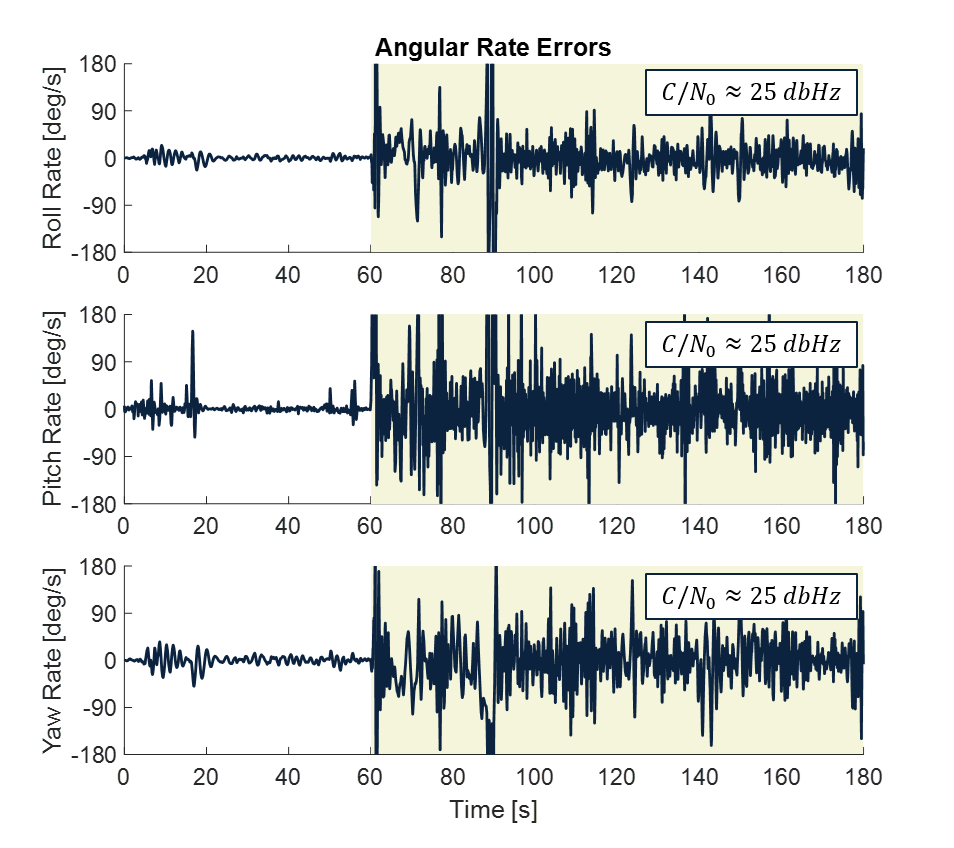
\includegraphics[width=0.75\linewidth]{Figures/Results/StraightAngularErrors.png}
    \caption{Angular Rate RMSE while subject to interference and flying steady, level, and with no acceleration.}\label{fig:SLUF}
\end{figure}


\section{\textbf{Future Work}}
For future work, the author recommends several items, both relating to the proposed navigation filter and to components of the FVDM presented in this work. In addition to the deeply-coupled FVDM with GPS correlator measurements, a recommendation is made to couple IMU or other external sensors with the FVDM for improvement in observability of angular rates and Euler angles. The addition of an IMU would provide a direct measurement of angular rates and specific forces that would correct the predicted forces and moments from the FVDM\@. This is especially beneficial in GPS-denied environments. The addition of a barometer would provide a direct measurement of pressure, which could be mapped to the altitude of the FVDM\@. The direct measurement of altitude would correct the FVDM in GPS-denied environments, and subsequently could provide an semi-observable mapping to pitch, pitch-rate, and the climb rate (\(V_D\)) of the FVDM\@. These recommendations stem from prior work performed by~\cite{khaghaniAssessmentVDMbasedAutonomous2018,khaghaniAutonomousVehicleDynamic2016,mwenegohaModelbasedTightlyCoupled2020} for loosely and tightly coupled architectures. Typically, real-world flying will not have standard-day atmospheric parameters as modeled during simulations presented in this work.  To better match actual atmospheric conditions, an implementation of a non-standard day atmospheric model is recommended. A comparative analysis of FVDM performance between the two atmospheric models is intriguing and is also recommended. For improvements to the vector tracking architecture, the author recommends implementation of a multi-signal vector tracking algorithm as seen in~\cite{givhanGPSL5Software2021}. The addition of another signal from a different constellation would increase the number of measurements greatly (especially if using a low-Earth orbit constellation). With modern signal modulation, the resistance to interference is increased, allowing vector tracking to retain channel lock even in scenarios of degradation.